\section{Data Processing}
\label{sec:dataProc}

This section covers the workflow to process the data produced by the DAQ system, illustrated in Fig.~\ref{fig:workflow}. The files written on the DAQ buffer disk are automatically transferred to offline storage, and the first reconstruction pass is run with the same conditions used by the trigger algorithms. Once completed, the calibrations constants are re-evaluated and updated in the conditions database. The main physics streams are then reprocessed using the latest conditions, and reduced datasets are finally produced for further analysis. These steps proceed in parallel: newer data are processed through the first reconstruction pass while older data are simultaneously reconstructed with the second reconstruction pass. The workflow is optimized to minimize the need to pre-stage files from tape and maximize the data throughput. Each stage is discussed in greater detail in the remainder of this section. 

\begin{figure}[ht!]
  \centering
  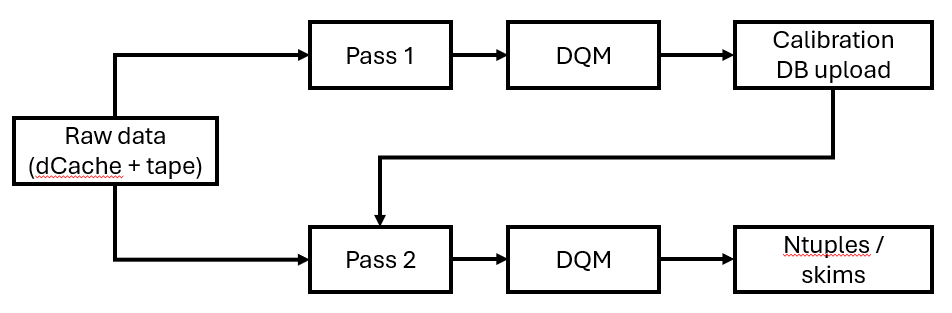
\includegraphics[width=0.95\textwidth]{figures/WorkflowOverview.png}
  \caption{Schematic of the Mu2e data processing workflow}
  \label{fig:workflow}
\end{figure}


\subsection{\passone}
\passone\ is the first stage, starting almost immediately after the data have been transferred from the DAQ buffer disks to dCache. It will process the totality of triggered events through the full set of offline reconstruction algorithms using the same conditions information used by the trigger algorithms. The following outputs will be produced:
\begin{enumerate}
 \item The main physics output file, which will contain events with signal-like tracks, for both $\mu^-\to e^-$ and $\mu^-\to e^+$, plus events of interest for background studies.
 \item Calibration files with events needed for the various calibration algorithms.
 \item Offline DQM information (see Section~\ref{sec:monitoring}) with higher statistics and more complete coverage than that provided by the online DQM system.
 \item Optionally, a file containing all data for debugging and validation purposes
\end{enumerate}
When necessary, the workflow will include stages to concatenate small output files into a single large file, e.g., off-spill events (there is a competing demand to produce prompt offline DQM information, and the optimal concatenation policy will be determined by the operational constraints).

Once a new run is started, the \passone\ workflow will start as soon as selected information from the online database is available offline. As the data logging system delivers files, the production system will monitor the file catalog and launch grid jobs to process new files (either a single or many files in one job). Under normal conditions, the jobs should be launched 10 minutes or less after the files have been cataloged and complete within 2 to 3 hours after submission. However, this time distribution is expected to have (long) tails during peak usage periods or if the system requires maintenance. Offline DQM information will be summarized in both timelines and metrics, and out-of-tolerance data will generate an alarm. The histograms and TTrees from which these metrics are derived will be retained on disk for a certain time and persisted on tape. Files in the Error/Debug stream will also be copied to tape, concatenated if necessary, and retained on disk for inspection by experts for a limited amount of time. 

The normalization file stream includes the Intensity stream and the summary data from the ExtMon and the STM. These streams contain information to evaluate the proton bunch intensity variations over the course of each spill. These data are needed to assess the reconstruction efficiency accurately and properly normalize the results. These streams have sparse per-event information (i.e. not all information is available for every event). In addition, packaging small data products as objects in an {\tt art::Event} is inefficient in both disk/tape space and access time. One possibility might be to organize the data around spills, and the resulting information could be persisted in a database or included in each art SubRun object. Final decisions will be taken as the design matures. For these files, \passone\ will package the information in a way that is convenient for downstream processing, and concatenate input files if necessary.

The first class of low-level calibration streams includes the prescaled raw and intermediate data from the monitors and the calorimeter pulser events. The corresponding \passone\ workflow will be defined by the detector teams, but the output should include DQM and updated condition information that will be uploaded to the condition database. The input files might only be stored in dCache for a limited amount of time. The second class of low-level calibration streams contains STM waveform data for pulses with energies near the important lines. The STM team plans to periodically refit these pulses with updated conditions information to improve the estimate of the stopped muon yield. This data will be written to tape, with file concatenation when necessary.


\subsection{Calibration}
The data workflow continues with the calibration step, using the data directly produced in \passone\ to update the detector calibration constants. A detailed description of calibration procedures is given in Section~\ref{sec:calibration}. Most of the time, the output of \passone\ should be sufficient to perform this work. However, it may be necessary to re-run a subset of \passone\ using the conditions information determined by the previous pass, and repeat the procedure until the calibration information has converged. This might be required, for example, during commissioning and early data taking. When necessary, the subsystem teams will be able to run repeated \passone\ jobs using the data production system, or by manual invocation of particular components ofit. Once calibrations are certified, the offline condition database is updated. The online condition database will be periodically synchronized to the offline database.


\subsection{\passtwo}
Once calibration constants for a time interval are certified, the main physics streams (on-spill and off-spill triggered events) are reprocessed using updated conditions information. This operation is called \passtwo\ and will produce a new set of DQM information and output data files. During commissioning and early data taking, \passtwo\ might perform the full reconstruction from the raw data. As we gain experience, it might become possible to only refit existing tracks and recalculate the parameters of existing calorimeter clusters and CRV stubs. In that case, the raw data in the output of \passone\ could be filtered to only include the necessary information.

Based on experience with previous experiments, Mu2e expects the following three-week cycle at the start of the experiment: during week N, take data for week N, run calibration jobs for data taken during week N-1, and run \passtwo\ for week N-2 data. As data taking becomes stable, it may be possible to compress this time scale. During a year-long run, we also expect continuous improvements in calibrations and reconstruction algorithms. When integrated improvements warrant it, we will re-run \passtwo\ on all recorded data. In this situation, a large dCache tape-backed volume and additional drives may be requested to speed up file pre-staging.  


\subsection{Reduced data sets}
The data workflow ends with the production of reduced data sets. The format and use cases are discussed in Section~\ref{sec:analysis}. There may be several types of datasets, each targeted to a particular analysis task. These data sets will be directly produced from the output of \passtwo, running additional reconstruction algorithms if needed. They will be produced for every iteration of \passtwo. As analysis algorithms evolve, reduced data sets will be reproduced to reflect these improvements. The output of \passtwo\ and reduced data sets should be small enough that this step will not require significant resources.

Additionally, skim data sets could also be produced from the output of \passtwo. Each skim data set contain a fraction of the original events, selected by a dedicated filter and preserving or augmenting content of the original event. These data sets would reduce computing needs and processing times during the analysis phase.   
